\documentclass[12pt,addpoints,answers]{guia}
\grado{2$^\circ$ de Secundaria}
\cicloescolar{2022-2023}
\materia{Ciencias y Tecnología: Física}
\guia{11}
\unidad{3}
\title{El Universo a simple vista}
\aprendizajes{\item Describe cómo se lleva a cabo la exploración de los cuerpos celestes por medio de la detección
de las ondas electromagnéticas que emiten.\item Describe algunos avances en las características
y composición del Universo (estrellas, galaxias y otros sistemas).}
\author{JC Melchor Pinto}
\begin{document}
\INFO%
\begin{sectionbox}{El Universo a simple vista}
    \begin{wrapfigure}[12]{r}[1mm]{0.35\textwidth}
        \centering
        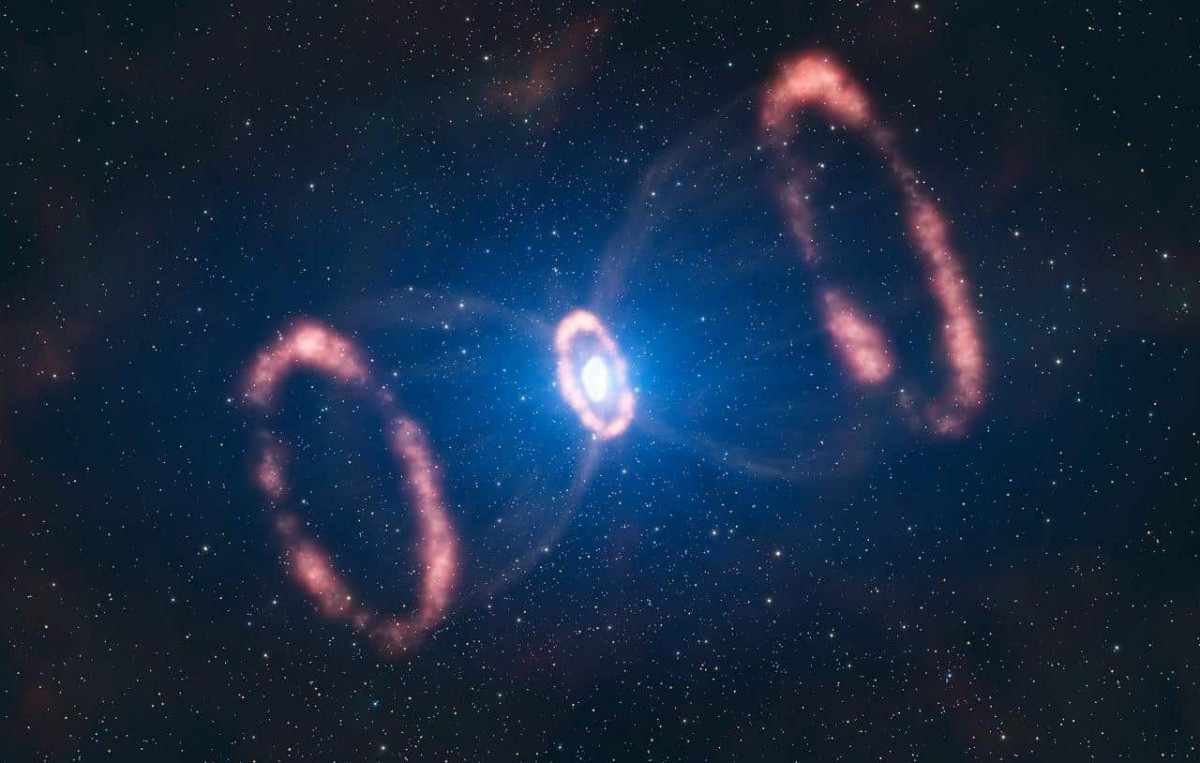
\includegraphics[width=\linewidth]{../images/supernova-default.jpg}
        \caption{Representación artística de la supernova SN 1987A.}
        \label{fig:supernova-default}
    \end{wrapfigure}

    ¿Cómo han descubierto los científicos la estructura del Universo que revisaste en la lección anterior? ¿Cómo saben
    los astrónomos a qué distancia está una galaxia y de qué está
    hecha? Quizá te has planteado preguntas de este tipo, y tal
    vez te sorprenda saber que con lo que aprenderás en este, tu
    primer curso de Física, obtendrás buenos conocimientos para
    responderlas, en su sentido más básico, claro.

    \begin{wrapfigure}[15]{l}[1mm]{0.25\textwidth}
        \centering
        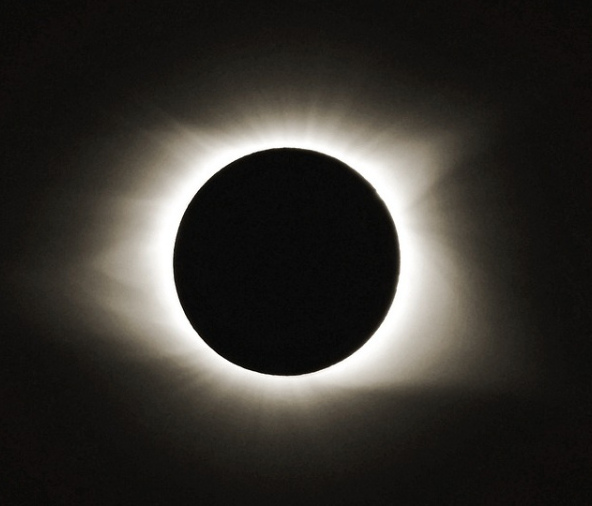
\includegraphics[width=\linewidth]{../images/eclipse-solar-total-mexico-2024.jpg}
        \caption{Fotografía de un eclipse solar al momento de la totalidad. La corona solar se observa levemente difuminada debido a la nubosidad parcial.}
        \label{fig:eclipse-solar-total-mexico-2024}
    \end{wrapfigure}

    El punto de partida para conocer el Universo fueron observaciones sencillas como las que mencionan los niños en el viejo
    cuento chino. Imagina que deseas visitar un pueblo o una ciudad por primera vez; entre
    lo primero que necesitamos saber para ir a ese lugar está averiguar dónde se ubica, cómo
    es, qué hay en él y en los alrededores. Algo similar hicimos los seres humanos, como especie para conocer el Universo. Así, aparte de explorar la Tierra, nuestros antepasados
    más antiguos miraron el cielo y comenzaron a registrar sus observaciones.



    A simple vista podemos distinguir el Sol, la Luna, algunos cometas, cinco planetas,
    unas seiscientas estrellas y en el hemisferio sur pueden verse las Nubes de Magallanes,
    que son dos galaxias. Ocasionalmente ha sido posible presenciar la explosión de alguna estrella, como las llamadas \textbf{supernovas} (figura \ref{fig:supernova-default}).



    Pero, ¿a qué distancia de nosotros están esos cuerpos
    celestes? En la vida cotidiana a cada momento estimamos distancias, calculamos lo lejos que está una persona
    a partir de su tamaño aparente. La perspectiva nos ayuda a estimar distancias: las casas lejanas, por ejemplo,
    parecen más pequeñas que las cercanas y el brillo de un
    objeto luminoso disminuye con la distancia. Nuestro cerebro infiere distancias todos los días al trabajar sobre
    nociones físicas o geométricas de las que somos poco
    conscientes.



    La siguiente noción es todavía más sencilla: si un objeto nos oculta la vista de otro, entonces está más cercano que el que oculta. Así, en un eclipse solar (figura \ref{fig:eclipse-solar-total-mexico-2024}) observamos no sólo que
    la Luna pasa delante del Sol, sino que, curiosamente, ambos tienen un tamaño en
    apariencia iguales. De ello derivamos, como lo hicieron nuestros antepasados, dos
    conclusiones: 1) El Sol está más lejos que la Luna, y 2) El Sol debe ser más grande que
    la Luna. Una observación similar permite comprender que el Sol está más cerca de
    nosotros que las estrellas.

    \begin{wrapfigure}[13]{l}[1mm]{0.35\textwidth}
        \centering
        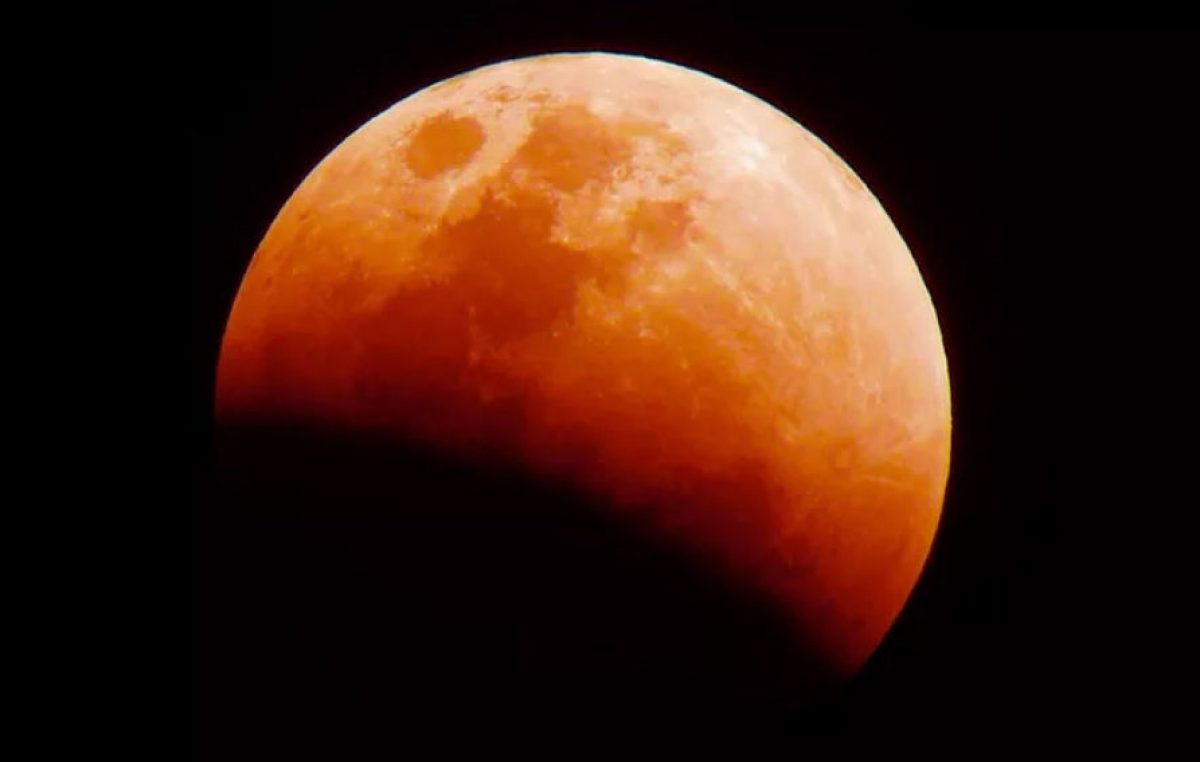
\includegraphics[width=\linewidth]{../images/eclipse-lunar-parcial.jpg}
        \caption{Sombra circular de la Tierra en los eclipses lunares.}
        \label{fig:eclipse-lunar-parcial}
    \end{wrapfigure}

    Conocer las distancias a las que están los cuerpos celestes cercanos fue el primer
    paso hacia el conocimiento del Universo. Esto se realizó sobre nociones sencillas pero
    con la ayuda de razonamientos sutiles, a veces muy ingeniosos, brillantes o definitivamente geniales.

    Los antiguos griegos encontraron razones para creer que la Tierra es redonda y sospechar que no es demasiado grande. Notaron que en mar abierto primero desaparece
    el casco y luego el velamen de las embarcaciones cuando se adentran en el mar, y que
    cuando se viaja de norte a sur, o viceversa, la altura aparente de las estrellas cambia. También comprendieron que los eclipses lunares
    se producen porque la Tierra se interpone entre el Sol y la Luna, y que la sombra de la Tierra proyectada sobre la Luna tiene siempre forma circular (figura \ref{fig:eclipse-lunar-parcial}).





    Hemos mencionado el método del que se valió
    Eratóstenes para determinar que la Tierra tiene una circunferencia
    de 252 000 estadios (40 000 km); otro griego, \textbf{Posidonio (135 a. n. e.-51 a. n. e.)}, también calculó la circunferencia de la Tierra. Al parecer comparó la altura de una estrella vista desde distintas ciudades,
    una más al sur que la otra. Aunque no existe registro exacto de su
    método, se sabe que estimó en 240 000 estadios (37 800 km) la circunferencia de nuestro planeta.

    \textbf{Aristarco de Samos (320 a. n. e.-250 a. n. e.)}, antes que Eratóstenes
    y Posidonio, consideraba que es la Tierra la que gira alrededor del
    Sol y no al revés, y desarrolló métodos muy ingeniosos para determinar las distancias y los radios del Sol y la Luna en términos del
    radio de la Tierra; sin embargo, no pudo calcular el radio de la Tierra, por lo que no conoció las dimensiones del Sistema Solar.
\end{sectionbox}
\begin{questions}
    \questionboxed[25]{\include*{../questions/question088a}}
    \questionboxed[25]{\include*{../questions/question088b}}
\end{questions}
\end{document}